\section{Libraries of additional pictures}
\label{sec:forsyde-pictures}

The \ForSyDeLaTeX\ utilities provide a set of additional libraries for drawing pictures used in related publications or documentation. These can be imported as regular \textsc{TikZ} libraries, in association with the \texttt{forsyde-tikz} package.
%
\begin{verbatim}
\usepackage[tikz]{forsyde}
...
\usetikzlibrary{library}
\end{verbatim}
%
\noindent where \texttt{library} is named along the lines of \texttt{forsyde.pictures.<name>}.

The following libraries are not extensively documented but rather listed along with the main commands and an example of usage. For more information check their source code.

\subsection{The \texttt{forsyde.pictures.layered} library}
\label{sec:forsyde-pictures-layered}

This library provides commands for depicting the concept of layered structure introduced in the \ForSyDeAtom\ project.

\begin{figure}[h]\hspace{-2ex}
  \centering
  \begin{minipage}{.68\linewidth}
  \lstinputlisting[linerange={9-30}]{figs_src/example-pictures-layered.tex}
\end{minipage}
~
\begin{minipage}{.3\linewidth}
  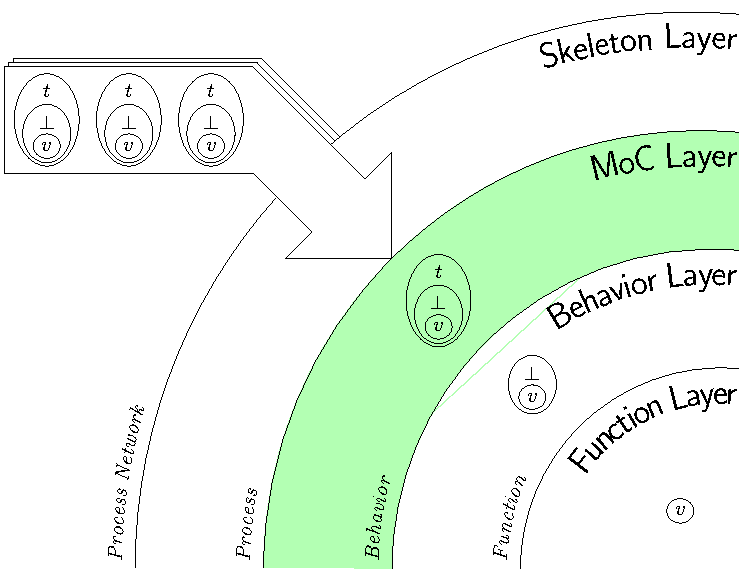
\includegraphics[scale=.4]{figs/example-pictures-layered}  
\end{minipage}
\end{figure}

\hspace{1pt}\bookmark{\char`\\forsydeAtomMakeLayers\opt{[options]}\man{\{list\_of\_layers\}}}

\noindent Creates a a picture of incremental layers wrapping each other, based on the list of labels, formatted in the following way:
%
\begin{verbatim}
  inner label 0: outer label 0, inner label 1: outer label 1, ...
\end{verbatim}
%
Each layer \texttt{N}, where $\mathtt{N} \in [0..n]$ has:

\begin{itemize}
\item a named referred to by other commands: \texttt{layerN};
\item defined coordinates/anchors: \texttt{layerN-center}, \texttt{layerN-left}, and \texttt{layerN-right};
\item defined paths: \texttt{layerN-leftpath} and \texttt{layerN-rightpath}.
\end{itemize}

\noindent The \texttt{options} are:

\begin{optionslist}
\item \texttt{width=} default is \texttt{3.8cm};
\item \texttt{height=} default is \texttt{1.8cm};
\item \texttt{length=} default is \texttt{1cm};
\end{optionslist}

\hspace{1pt}\bookmark{\char`\\forsydeAtomSignalArrow\opt{[options]}\man{\{position\}}}

\noindent Creates a a picture of wide arrow representing signal of events. The \texttt{position} is where the arrow tip should point to. It has defined the following coordinates/anchors: \texttt{arrow-south}, \texttt{arrow-north}, \texttt{arrow-east}, \texttt{arrow-west}, \texttt{arrow-center}. The \texttt{options} are:

\begin{optionslist}
\item \texttt{left indent=} default is \texttt{3pt};
\item \texttt{right indent=} default is \texttt{0pt};
\item \texttt{label shift=} default is \texttt{-4ex};
\item \texttt{layer radius=} default is \texttt{2cm};
\end{optionslist}

\hspace{1pt}\bookmark{\char`\\forsydeAtomSignalVector\man{\{interesction\_path\}}}

\noindent Is used after a \texttt{\char`\\forsydeAtomSignalArrow} command to draw at which layer \texttt{interesction\_path} does a signal is transformed into a structure/vector of signals.

\vspace{1ex}
\hspace{1pt}\bookmark{\char`\\forsydeAtomHighlightLayer\opt{[color]}\man{\{layer\_number\}}}

\noindent Highlights a layer by filling it with a background color. Default \texttt{color} is \texttt{red}.

The  \texttt{forsyde.pictures.layered} library also holds a number of shapes defined as \texttt{box}es. These boxes are:

\begin{itemize}
\item \texttt{\char`\\forsydeAtomValue}
\item \texttt{\char`\\forsydeAtomExtValue}
\item \texttt{\char`\\forsydeAtomTagValue}
\item \texttt{\char`\\forsydeAtomTagExtValue}
\end{itemize}


%%% Local Variables:
%%% mode: latex
%%% TeX-master: "../refman"
%%% End:
